\section{Hierarchical Clustering} \label{hierarchicalClustering}
\subsection{Introduction}
Hierarchical clustering, also known as connectivity based clustering, was the next applied approach. This area of algorithms clusters nodes together, which are near to each other. The advantage over K-Means is that graph distances can be used instead of the euclidean distance.

The result of a hierarchical clustering algorithm is a tree (or hierarchy), hence the name. This result can be used to create 1 to n clusters, where n is the number of input nodes.

\subsection{Strategy}
There are generally two main strategies for hierarchical clustering:

\begin{itemize}
    \item \textbf{Agglomerative}: Bottom up strategy. In the beginning each node is an own cluster. Clusters are combined until only a single cluster remains.
    \item \textbf{Divisive}: Top down strategy. All nodes are contained in one cluster at the start. This cluster is then divided into sub clusters.
\end{itemize}

The time complexity of the divisive strategy with $O(2^n)$ is too bad for the size of the street networks on which the algorithms have to run. The agglomerative strategy runs in $O(n^2 log(n))$ and in some special cases in $O(n^2)$ time complexity. The hierarchical clustering algorithms implemented for this thesis run in $O(n^2)$ time complexity. They are based on the paper "Optimal implementations of UPGMA and other common clustering algorithms" \cite{clustering:2007}.

\subsection{Reduction Formula}
The reduction formula is used to determine the distance between two clusters.
The following reduction formulae were implemented for this thesis:

\begin{itemize}
    \item \textbf{Single Linkage}
    \begin{multline}
    D_{Single-Linkage}(C_1, (C_2 \cup C_3)) \leftarrow \\
    min \{ D_{Single-Linkage}(C_1, C_2), D_{Single-Linkage}(C_1, C_3) \}
    \end{multline}
    \item \textbf{\acrshort{UPGMA}} (\acrlong{UPGMA})
    \begin{equation}
    \begin{split}
    D_{UPGMA}(C_1, (C_2 \cup C_3)) \leftarrow &\frac{|C_2|}{|C_2|+|C_3|}D_{UPGMA}(C_1, C_2)\ + \\ &\frac{|C_3|}{|C_2|+|C_3|}D_{UPGMA}(C_1, C_3)
    \end{split}
    \end{equation}
    \item \textbf{\acrshort{WPGMA}} (\acrlong{WPGMA})
    \begin{equation}
    D_{WPGMA}(C_1, (C_2 \cup C_3)) \leftarrow \frac{1}{2} (D_{WPGMA}(C_1, C_2) + D_{WPGMA}(C_1, C_3))
    \end{equation}
\end{itemize}

With clusters $C_1$, $C_2$ and $C_3$, which are sets of nodes and the distance function $d(i, j)$, which determines the distance between nodes $i$ and $j$.

For every of these reduction formulae the following holds:

\begin{equation}
\begin{split}
&\textrm{let }C_1, C_2\textrm{ be clusters}, i \in C_1, j \in C_2 \\
&\textrm{if }|C_1| = |C_2| = 1 \\
&\textrm{then }D(C_1, C_2) = d(i, j)
\end{split}
\end{equation}

For both the single linkage and the \acrshort{UPGMA} reduction formula exists a dissimilarity function (\ref{eq:df_single_linkage} and \ref{eq:df_upgma}). These are alternative formulations of the reduction formulae which determine the distance by traversing all nodes of both clusters. The created cluster hierarchy is not used in these functions. For the \acrshort{WPGMA} reduction formula no dissimilarity function exists, as shown in \cite{clustering:2007}.

\begin{equation} \label{eq:df_single_linkage}
D_{Single-Linkage}(C_1, C_2) = \min_{i\in{C1}, j\in{C2}}\{d(i, j)\}
\end{equation}
\begin{equation} \label{eq:df_upgma}
D_{UPGMA}(C_1, C_2) = \dfrac{1}{|C_1||C_2|} \sum_{i\in{C1}, j\in{C2}}{d(i, j)}
\end{equation}

\subsection{Single-Linkage Result}
The figure \ref{fig:SingleLinkage} shows the result of a hierarchical cluster analysis using the single linkage reduction formula. The used distance function $d(i, j)$ was the shortest distance from $i$ to $j$ in the street graph. As it is clearly visible when looking at the result, this way of cluster analysis is not creating the desired output. There is one huge cluster in the middle and many one-node clusters at the border of the city.

The problem is caused by the used reduction formula. Single linkage uses the distance between the closest nodes of the compared clusters. This leads to the creation of clusters, where all connecting roads are long. In a city, where there are multiple connections from one junction to another most of the time, this tends to create one-node clusters for nodes, which are connected to the city by a single long road.

\begin{figure}[!h]
    \centering
    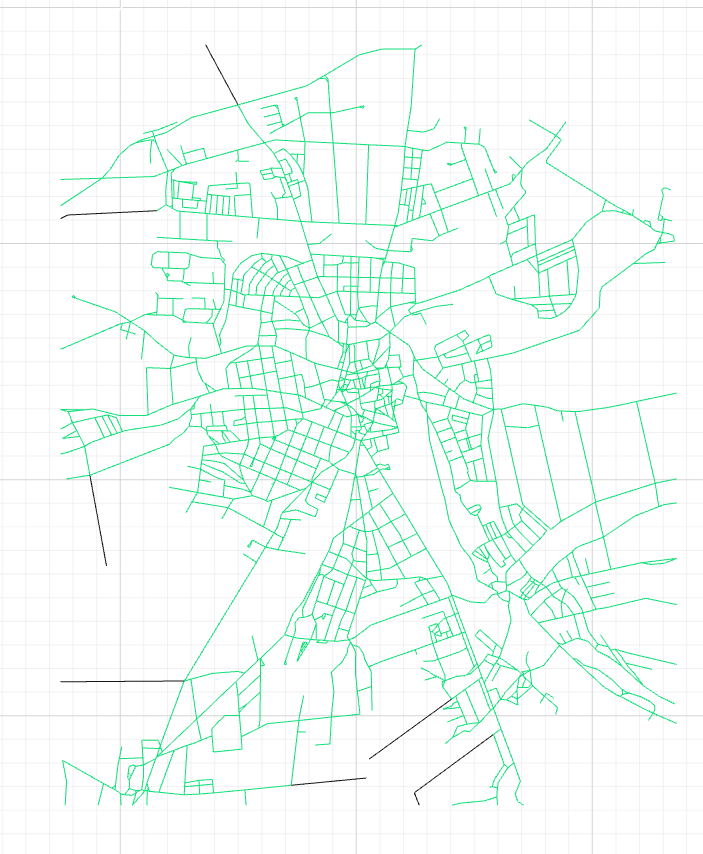
\includegraphics[width=\textwidth]{clusteranalysis_singlelinkage.png}
    \caption{Single-Linkage hierarchical cluster analysis of Weimar\label{fig:SingleLinkage}}
\end{figure}

\subsection{UPGMA and WPGMA Result}
\label{sec:UPGMAandWPGMA}
%TODO: Add figure
The figures xxx and xxx show the result of hierarchical cluster analysis using the \acrshort{UPGMA}, or respectively the \acrshort{WPGMA} reduction formula. The same distance function $d(i, j)$ as in the single linkage solution was used (shortest distance from $i$ to $j$ in the street graph).

\subsection{All Pairs Shortest Path}
As already stated, the implementations of hierarchical clustering algorithms developed during this thesis use graph distances. The calculation of the shortest path between two nodes every time it is needed would not be viable, because these distances have to be accessed multiple times. So it is necessary to calculate and store them in advance using an \gls{APSP} algorithm.
%TODO: FW, Dijkstra, FW_GPU?

\subsection{Memory usage}
The most trivial solution would be to store the distances as a matrix of double-precision floating-point numbers. This is because the given numeric data was already in this number format and a matrix is easily accessible. For \acrshort{UPGMA} and \acrshort{WPGMA} this matrix has to be extended so it also includes the cached distances between clusters.

This storage strategy would use $(2n-1)^2$ double-precision floating-point numbers, $n$ being the node count (number of junctions). As an example: For the used environment this storage strategy would amount to about 21.7 Gigabyte of used memory for the street network of Zurich.

The easiest optimisation is to convert all distances to a single-precision floating-point format. The loss of precision is not affecting the result, as mostly only the $<$ and $>$ relations of the different distances are important.

A second optimisation that can be applied is, to remove redundant information. When storing the full matrix of all distances, most values are stored twice. The matrix is mirrored along the diagonal, because the used street networks are undirected graphs. So the memory usage can almost be cut in half if those duplicates are not stored.

The third and last applied optimisation was to change the way, how cluster distances are stored if the reduction formula \acrshort{UPGMA} or \acrshort{WPGMA} is used. Each time, when two clusters are combined, the distances of the new formed cluster to every other cluster are calculated. This combination step is done using the distances stored for the two old clusters. Afterwards the distances which were stored for the old clusters are no longer used. To reduce the memory usage, the distances of the new cluster can therefore be stored, at the location where the distances of one of the old clusters were stored.

\subsection{Output Modification}
- Equalization of cluster sizes
%TODO: Write subsection & Add images
